\documentclass[a4paper, 11pt]{article} % Font size (can be 10pt, 11pt or 12pt) and paper size (remove a4paper for US letter paper)

\usepackage{../essay}
\usepackage{pdfpages}
\graphicspath{ {../img/}{../../img/} }

\begin{document}

\textit{The following is taken from an essay I wrote in August 2016. This is a portion of the first chapter of a write-up reflecting on the experience of attending SIGGRAPH 2016 as a student volunteer. My hope is that this excerpt explains Chris Tralie's role as a mentor who was directly responsible for my having grown as a student and life-long learner while I was a senior enrolled in his class. The purpose of including this is to provide a context for my statement of support for my student nominee for the Dean's Award of Excellence in Mentoring. Chris Tralie was my instructor for a course in Digital 3D Geometry, taught under the Duke University Bass Family Teaching Fellowship during the Spring 2016 semester.}
	
\bigskip

The entire write-up can be found at the following link:

\begin{center}
\url{https://github.com/bmershon/siggraph-2016}
\end{center}

\begin{center}
	\textellipsis
\end{center}

Pacing back and forth in front of the class, sweating in the humid math building during one of the scheduled lectures for MATH 412, Chris excitedly painted a picture of his work and the applications of your course to his own research. He was raring for the opportunity to share his unique insights into connections between digital signal processing, computational geometry, and his own mathematical scaffolding he has constructed as he paved his way through academia. His whole life he has been a hacker. He was by now coming into his own as a teacher and academic as well. It is no surprise that he was awarded a teaching fellowship the following year---your senior year---which would allow him to serve as the instructor for a course of over 40 students with a curriculum entirely of his own design.
 
When you see that Chris is teaching \textit{Digital 3D Geometry} in the Spring of your senior year, you check your clunky online portal to see if CS/MATH 290 happens to fit in your gridlocked schedule. It does, but it will be your fifth course, usually considered overloading at your university. You show up for the second lecture and talk to the instructor after class, inquiring about auditing the course. He remembers you and expresses how much he would enjoy having you in his course, reminding you that he would not be able to give you as much attention during office hours to help with projects if you audit. The projects are where the real learning takes place, and you know you are going to want attention and help, so you enroll.

CS 290 quickly becomes your top priority. It is a class in which every lecture is a whirlwind sojourn into an entirely new slice of Chris's research, with small pillars of theoretical fundamentals erected only as they are needed. The first few lectures cover vectors, dot products, and notions of duality in geometry. The next few weeks after that involve matrix operations and a significant project on ray tracing and scene graphs. At some point you learn about quaternions. Then you leap to statistics which can be performed on point clouds to categorize shapes. You learn how to do linear algebra quite quickly with Python and you begin to wrestle with high-dimensional data analysis. Eventually, topology creeps up and you encounter the Euler characteristic, followed by a brief intro to data structures for geometry. Near the very end, you learn about Chris's connections made between geometry and his deep study of digital signal process.

\begin{figure}[h!]
	\centering
	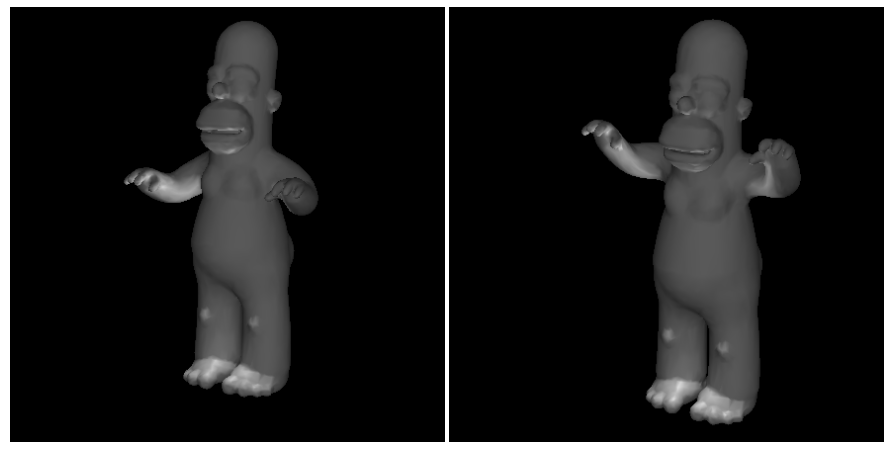
\includegraphics[width=\textwidth]{homer}
	\caption*{Laplacian mesh editing in Chris Tralie's course.}
\end{figure}

There are countless positive memories you have from his class in which you felt you truly learned something through experience that cannot be read out of a textbook. One morning found you struggling to debug a recursive ray-tracing algorithm that you were implementing. You had chosen to dive head first into an ambitious project the had set up for the class, striving to achieve one of the first milestones as soon as possible because you knew subsequent tasks would only be harder and more prone to set backs. In the back of your mind you were always concerned that you might suddenly let him down, that something would suddenly become too difficult and you would not be up to snuff. Chris was so pleased at your efforts to make a dent in his project that he held office hours remotely in the middle of a snow storm, working with you over Google Hangouts as you were cooped up in a library to debug your code. Early on you established that you would give your all in his projects and work closely with him to provide feedback and often times help relieve his work load by your very catching of problems with an assignment before an entire class was confused and against a deadline. 

\begin{figure}[h!]
	\centering
	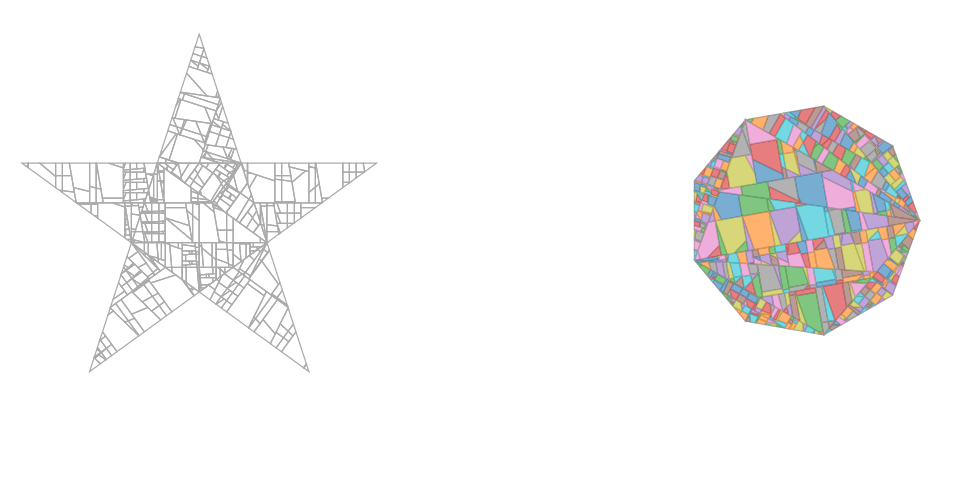
\includegraphics[width=\textwidth]{star-to-nonagon-teaser}
	\caption*{Equidecomposability: Final project for Chris Tralie's course.}
\end{figure}

While you are among the stronger students in the class, it is not your programming ability that Chris respects in you or your mathematical aptitude, but rather your ability to work hard and honestly in return for his hard work and effort put into producing a fantastic learning experience. Chris has made it clear early on that he respects hard work and detests what he calls "genius worship." You are \textit{in the mix} as he says, and so long as you keep eagerly doing everything you can to improve and learn in his course, you are doing things right in his mind. You have enough ability to do the work and have an attitude about learning that meshes well with his own. You respect his willingness to balance being a full-time graduate student with never failing to deliver a well-prepared lecture and projects which sometimes take 10 to 20 hours for him to design and produce boilerplate code for. While you are just another one of his students, and you are sure to respect this arrangement, you are also close during office hours, talking through more than just the material you are learning and hiccups related to a recent assignment. You talk about work habits, about his good and bad experiences in academia, about working with team members, about organizing your time, about dealing with anxiety, about relationships, about what it means to balance studying math with living your own life. Chris is your senior, but he is still only 27 years old.

Fairly early on in the semester, Chris announces to the class that SIGGRAPH accepts student volunteers. He encourages you all to apply and by this time he knows you well enough to happily write a letter of recommendation for you. For this, and for the subsequent letters of recommendations that he has written, you are extremely grateful. Chris was first a student, then an instructor, and then a friend to you. He was a mentor like the few other exceptional people you have had as professors during your undergraduate career. Chris admits to you that his knowledge of the industry is nearly nonexistent, perhaps willfully so! Chris can coach you on entering academia, but when it comes to figuring out what to do after college, SIGGRAPH is probably one of your best bets for meeting potential employers and ideally discovering something you love that you had not previously known even existed. Chris is excited for you and really hopes to see you find something you enjoy. You fill out the information required, answer a few behavioral questions, and provide Chris's contact info in your online application. Then you wait until late April to see if you'll be going to Anaheim.

\begin{figure}[h!]
	\centering
	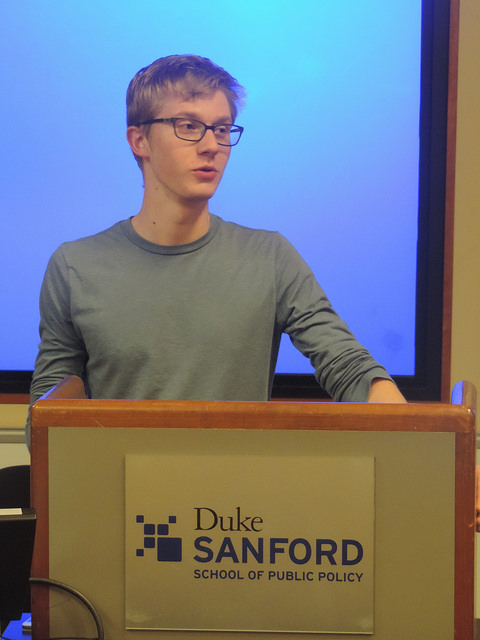
\includegraphics[width=0.5\textwidth]{ted_talk}
	\caption*{Mock Ted Talk: Paper, Pencil, Program.}
\end{figure}

It is worth noting that while your junior year was heavily influenced by your course with Paul Bendich and your senior year ended with a string of significant coursework in Chris's class of which you are quite proud, there is one other character who very much has pushed in in the right directions, acting as a mentor and showing you what is possible. Justin Curry, only 28 years old when he was an assistant professor at Duke and your instructor in a course in linear programming, is one of those people who you will never forget. Paul and Chris know Justin because he too works in the field of topology. To put things simply, when you were tasked with delivering a mock Ted Talk in your public speaking class during your second semester of senior year, you could not think of any story more worthy of sharing than the one that tells of how these three mentors had a great impact on your. All this is to say, you are headed to SIGGRAPH on account of a few mentors you lucked out into crossing paths with in college. Chris is perhaps most directly responsible for your journey to SIGGRAPH, but these three figures are connected in your mind. The actual outline you wrote for mock TED Talk is included on the next page. It more or less contains the best of what the second half of your undergraduate career brought you.

Going into SIGGRAPH, the only thing that will have changed since you were in Chris's class is the need for a job. In fact, you have been humbled by the search for a job and are all the better for having worked to finally arrive at a place where you are happy and feel you can learn. The next step after college wasn't as obvious as the step \textit{into} college. With that worry out of the way, you are free to focus on seeing what it is that other folks are doing in the field of computer graphics. Your goal is to observe and absorb. Funnily enough, Chris's class took such an odd tour through interrelated topics in computational geometry that what it means to actually render geometric models on the screen barely came up in the course. You certainly are not walking into SIGGRAPH with the same culture that most of the artistically-inclined students will share. You know SIGGRAPH will be wonderful and probably worthwhile, but beyond that you know little about what to expect.

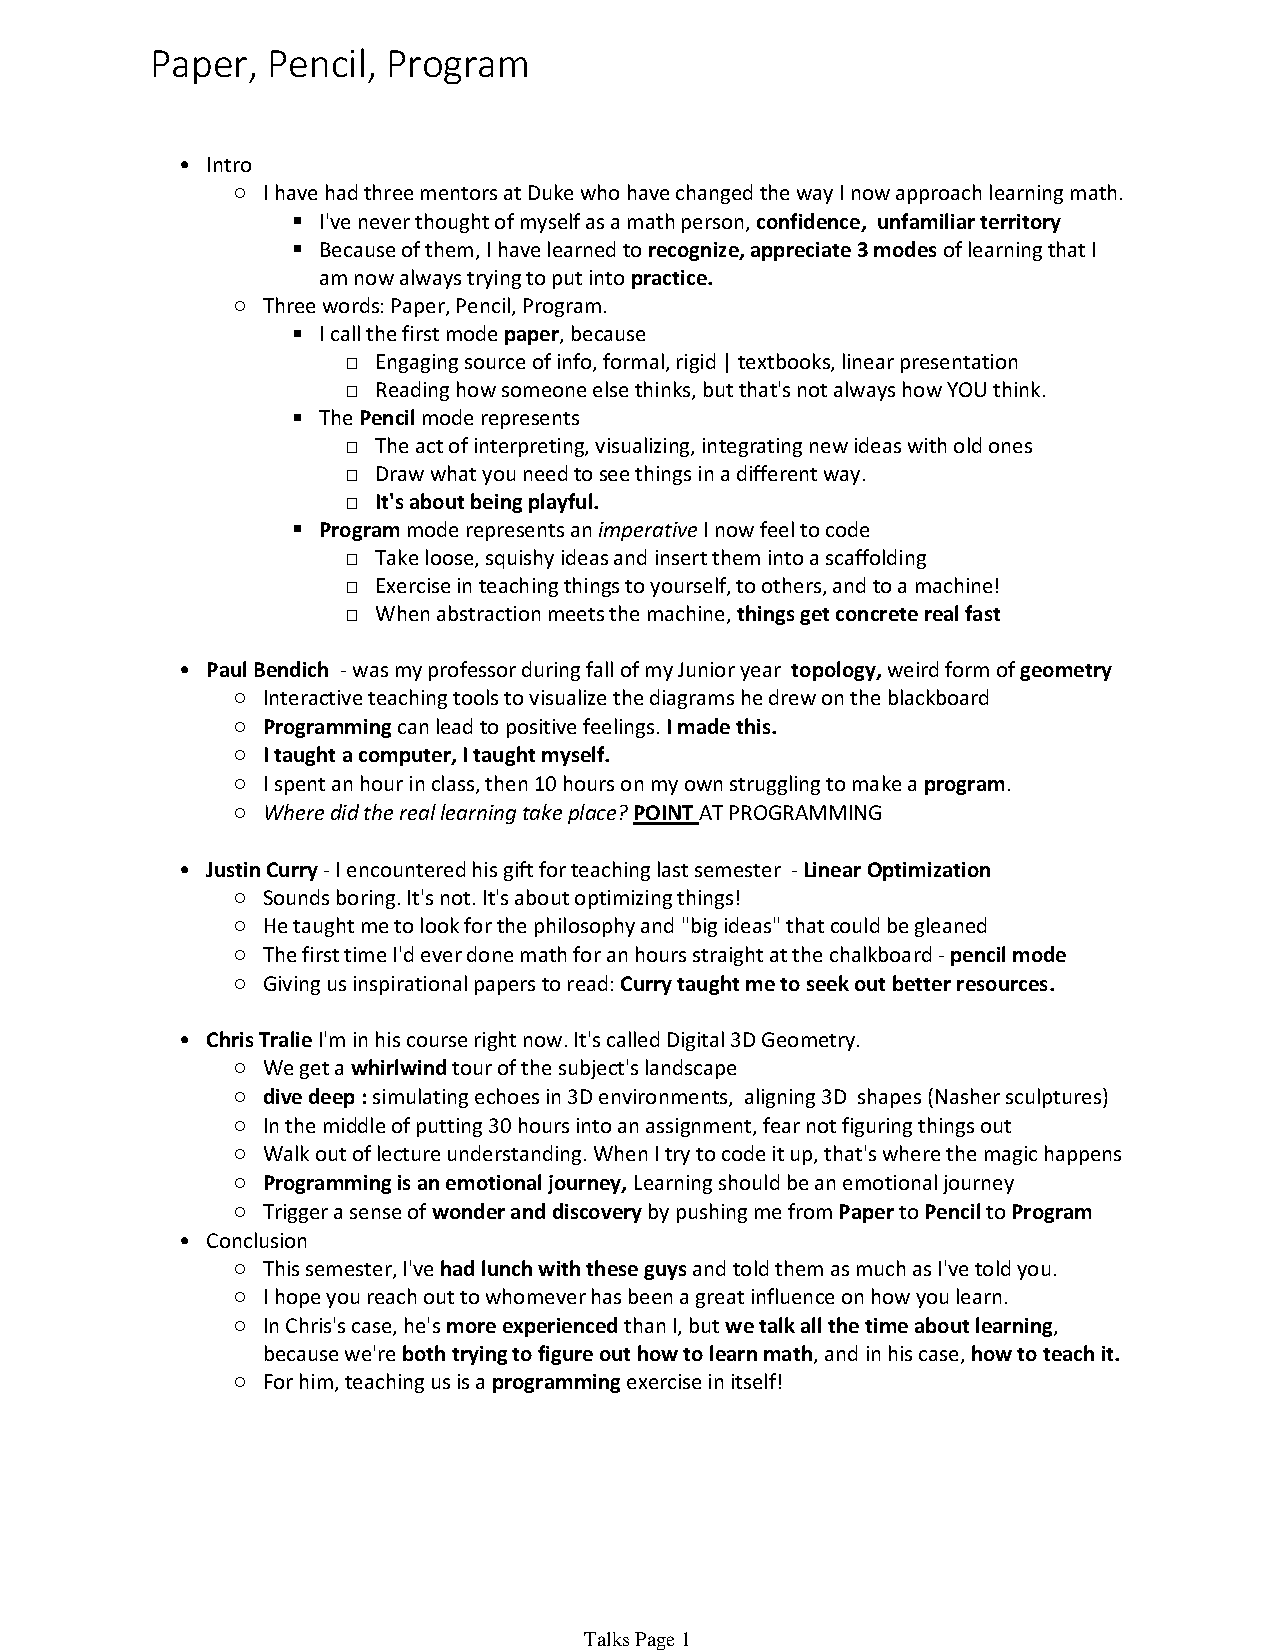
\includepdf[pages=-]{../external/paper-pencil-program.pdf}

\end{document}